\documentclass[aspectratio=169]{beamer}

\usetheme{CambridgeUS}
\usecolortheme{beaver}

% --- U of T BRAND COLORS (same as other CSC415 lectures) ---
\definecolor{UofTBlue}{RGB}{0, 42, 92}
\definecolor{UofTSky}{RGB}{0, 127, 163}
\definecolor{UofTSilver}{RGB}{226, 231, 235}

\setbeamercolor{palette primary}{bg=UofTBlue, fg=white}
\setbeamercolor{palette secondary}{bg=UofTSky, fg=white}
\setbeamercolor{palette tertiary}{bg=UofTBlue, fg=white}

\setbeamercolor{title}{bg=UofTBlue, fg=white}
\setbeamercolor{subtitle}{fg=UofTSilver}
\setbeamercolor{frametitle}{bg=white, fg=UofTBlue}
\setbeamercolor{structure}{fg=UofTBlue}
\setbeamercolor{item}{fg=UofTSky}

\setbeamercolor{block title}{bg=UofTBlue, fg=white}
\setbeamercolor{block body}{bg=UofTSilver, fg=black}

\setbeamertemplate{headline}{
  \begin{beamercolorbox}[ht=3.5ex,dp=1.125ex,leftskip=12pt,rightskip=12pt]{section in head/foot}
    \usebeamerfont{section in head/foot}\insertsection
  \end{beamercolorbox}
}

\setbeamertemplate{navigation symbols}{}

\usepackage{amsmath}
\usepackage{amssymb}
\usepackage{graphicx}
\graphicspath{{./}{media/}{images/}{../logo/}}
\usepackage{hyperref}
\usepackage{booktabs}
\usepackage{caption}
\usepackage{natbib}
\setbeamerfont{caption}{size=\footnotesize}
\usepackage{tikz}
\usetikzlibrary{arrows.meta, positioning, calc, decorations.pathreplacing}

\title[Adaptive Chunk Execution]{Inference-Time Adaptive Execution for Transformer Action Chunking}
\subtitle{CSC415 Course Project Final Presentation}
\author{Zuhayr Ahmed \and Charles Cheung \and Lawrence Fu}
\institute[]{CSC415: Introduction to Reinforcement Learning}
\date{April 2026}

\makeatletter
\setbeamertemplate{title page}{
  \vbox{}
  \vfill
  \begingroup
    \centering
    \IfFileExists{../logo/uoft.png}{%
        \includegraphics[width=0.25\textwidth]{../logo/uoft.png}%
    }{%
        \textcolor{UofTBlue}{\textbf{University of Toronto}}%
    }\\[1.5em]
    \begin{beamercolorbox}[sep=12pt,center,rounded=true,shadow=true]{title}
      \usebeamerfont{title}\inserttitle\par%
      \ifx\insertsubtitle\@empty%
      \else%
        \vskip0.5em%
        {\usebeamerfont{subtitle}\usebeamercolor[fg]{subtitle}\insertsubtitle\par}%
      \fi%
    \end{beamercolorbox}%
    \vskip1em\par
    {\usebeamerfont{author}\insertauthor}\vskip0.5em
    {\usebeamerfont{institute}\insertinstitute}\vskip0.5em
    {\usebeamerfont{date}\insertdate}\vskip0.5em
  \endgroup
  \vfill
}
\makeatother

% Optional: section divider slides (see lecture10.tex for \sectionbanner{...} example)
% Task stills: latex/media/lift.png, can.png, square.png (compile from latex/).

\newcommand{\resulttaskrow}{%
  \begin{center}
    \scriptsize
    \setlength{\tabcolsep}{8pt}%
    \begin{tabular}{@{}c@{\hspace{1em}}c@{\hspace{1em}}c@{}}
      \IfFileExists{media/lift.png}{\includegraphics[height=0.11\textheight,keepaspectratio]{media/lift.png}}{\fbox{\tiny lift}} &
      \IfFileExists{media/can.png}{\includegraphics[height=0.11\textheight,keepaspectratio]{media/can.png}}{\fbox{\tiny can}} &
      \IfFileExists{media/square.png}{\includegraphics[height=0.11\textheight,keepaspectratio]{media/square.png}}{\fbox{\tiny sq.}} \\
      Lift & Can & Square \\
    \end{tabular}
  \end{center}
  \vspace{0.2em}
}

\begin{document}

{
\setbeamertemplate{footline}{}
\frame{\titlepage}
}

\begin{frame}{Contents}
    \begin{itemize}
        \item Background
        \item Motivation
        \item Research gap \& project aim
        \item Methodology
        \item Experimental setup
        \item Results \& discussion
        \item Limitations and future work
    \end{itemize}
\end{frame}

\section{Background}
\begin{frame}{Background}
    \begin{itemize}
        \item \textbf{Action Chunking with Transformers} by \cite{zhao2023} is a method that combines transformers (CVAE) and action chunking for great long-horizon performance and stability.
        \item \textbf{RoboMimic} is a suite of exercises centered around simulating a robotic manipulator arm around various tasks
    \end{itemize}
\end{frame}

\section{Motivation}
\begin{frame}{Motivation}
    \begin{itemize}
        \item Action Chunking provides temporal abstraction by predicting $k$ future actions at
once instead of predicting single actions, which reduces the length of the horizon by $k$ times.
        \item Transformer action chunking improves long-horizon control, but fixed chunk length can reduce reactivity near contact events.
        \item Real-time execution can show chunk-boundary inconsistency/jitter under latency and uncertainty.
        \item We focus on \textbf{inference-time execution policy}: when should a chunk be preempted and replanned?
        \item Goal: improve success/reactivity tradeoff without changing simulator dynamics or requiring extra labels.
    \end{itemize}
\end{frame}

\section{Research gap \& project aim}
\begin{frame}{Research gap \& project aim}
    \begin{itemize}
        \item Prior chunking methods usually fix execution horizon or use smoothing, but do not deeply study adaptive commits in our low-dim RoboMimic setup.
        \item We propose \textbf{adaptive commit-length} execution using disagreement / delta / uncertainty rules.
        \item Core hypothesis: adaptive execution can match or improve rollout quality while reducing unnecessary replans.
    \end{itemize}
\end{frame}

\section{Methodology}
\begin{frame}{Methodology}
\begin{columns}[T,onlytextwidth]
\begin{column}{0.52\textwidth}
    \begin{itemize}\footnotesize
        \item ACT policy predicts a chunk $(a_t,\ldots,a_{t+k_{\max}-1})$.
        \item Executor holds a \textbf{FIFO} action queue; commit length $m\in[k_{\min},k_{\max}]$.
        \item \textbf{Overlap disagreement:} compare the still-queued tail with the overlapping prefix of the \emph{new} chunk; if they disagree enough, \textbf{preempt} and replan.
        \item Ablations: action-change threshold, stochastic uncertainty threshold.
        \item Temporal ensembling included as a comparator.
    \end{itemize}
\end{column}
\begin{column}{0.46\textwidth}
    \centering
    \vspace{-0.2em}
    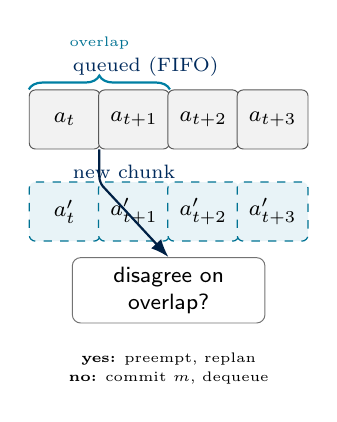
\begin{tikzpicture}[
      font=\sffamily\footnotesize,
      >=Latex,
      actQ/.style={draw=black!65, line width=0.35pt, rounded corners=2.2pt,
        minimum width=9mm, minimum height=7.5mm, inner sep=0pt, fill=black!5},
      actN/.style={draw=UofTSky!90!black, dashed, line width=0.45pt, rounded corners=2.2pt,
        minimum width=9mm, minimum height=7.5mm, inner sep=0pt, fill=UofTSky!9},
      hdr/.style={font=\scriptsize, text=UofTBlue, anchor=west}
    ]
      \def\dx{0.88}
      % Aligned indices (matches code: compare first $m$ steps of queue vs candidate; figure shows $m=2$).
      \node[hdr] at (-0.02, 1.72) {queued (FIFO)};
      \node[actQ] (q0) at (0, 1.05) {$a_{t}$};
      \node[actQ] (q1) at ({\dx}, 1.05) {$a_{t+1}$};
      \node[actQ] (q2) at ({2*\dx}, 1.05) {$a_{t+2}$};
      \node[actQ] (q3) at ({3*\dx}, 1.05) {$a_{t+3}$};
      \node[hdr] at (-0.02, 0.38) {new chunk};
      \node[actN] (n0) at (0, -0.12) {$a'_{t}$};
      \node[actN] (n1) at ({\dx}, -0.12) {$a'_{t+1}$};
      \node[actN] (n2) at ({2*\dx}, -0.12) {$a'_{t+2}$};
      \node[actN] (n3) at ({3*\dx}, -0.12) {$a'_{t+3}$};
      \draw[thick, UofTSky, decorate, decoration={brace, amplitude=5pt, mirror}]
        (q1.north east) -- (q0.north west)
        node[midway, above=0.38cm, font=\tiny, text=UofTSky!90!black] {overlap};
      \node[draw=black!55, rounded corners=3pt, line width=0.35pt, fill=white,
            align=center, inner sep=3.5pt, text width=22mm]
        (dec) at ({\dx*1.5}, -1.12) {disagree on overlap?};
      \coordinate (split) at ($(q0.south east)!0.5!(q1.south west)$);
      \draw[->, thick, UofTBlue!75!black, rounded corners=2pt]
        (split) -- ($(split)+(0,-0.42)$) -- (dec.north);
      \node[below=2.5mm of dec, font=\tiny, align=center, anchor=north]
        {\textbf{yes:} preempt, replan\\[1pt]\textbf{no:} commit $m$, dequeue};
    \end{tikzpicture}
\end{column}
\end{columns}
\end{frame}

\section{Experimental setup}
\begin{frame}{Experimental setup}
    \begin{itemize}
        \item Tasks: RoboMimic low-dim Lift, Can, Square.
        \item ACT-Strong config shared across tasks; matched eval protocol.
        \item Baselines: BC-MLP, kNN-BC (VINN-style), BeT-style discrete BC.
        \item Metrics: success, return, policy queries, replans/episode, commit statistics.
        \item Rigor: ablations + 3-seed runs.
    \end{itemize}
\end{frame}

\section{Results \& Discussion}
\begin{frame}{ACT-Strong results (cross-task)}

\begin{columns}[T]

% --- LEFT: TABLE + TEXT ---
\begin{column}{0.5\textwidth}
    \scriptsize
    \begin{tabular}{lcc}
    \toprule
    Task / mode & Success & Return \\
    \midrule
    Lift dynamic & 1.00 & 60.00 \\
    Lift temporal ensemble & 1.00 & 76.10 \\
    Can dynamic (z0) & 0.50 & 144.90 \\
    Can temporal ensemble (z0) & 1.00 & 289.15 \\
    Square dynamic (z0) & 0.15 & 42.05 \\
    Square receding (z0) & 0.20 & 41.70 \\
    \bottomrule
    \end{tabular}

    \vspace{0.4em}

    \begin{itemize}
        \item Lift strongly supports adaptive execution.
        \item Can is mixed and setting-sensitive.
        \item Square is challenging.
    \end{itemize}
\end{column}

% --- RIGHT: IMAGES ---
\begin{column}{0.3\textwidth}
    \centering
    \includegraphics[height=0.21\textheight]{../media/lift.png}\\
    {\tiny Lift}

    \vspace{0.05em}

    \includegraphics[height=0.21\textheight]{../media/can.png}\\
    {\tiny Can}

    \vspace{0.05em}

    \includegraphics[height=0.21\textheight]{../media/square.png}\\
    {\tiny Square}
\end{column}

\end{columns}

\end{frame}

\begin{frame}{Baseline summary (receding-horizon eval)}
\footnotesize
\begin{tabular}{@{}lcc@{}}
\toprule
Task / baseline & Success & Return \\
\midrule
Lift BC / kNN / BeT & 0.65 / 0.75 / 0.75 & 70.7 / 44.4 / 127.3 \\
Can BC / kNN / BeT & 0.00 / 0.30 / 0.30 & 0.0 / 58.65 / 33.75 \\
Square BC / kNN / BeT & 0.05 / 0.35 / 0.05 & 0.3 / 43.0 / 5.6 \\
\bottomrule
\end{tabular}
\vspace{0.5em}
\begin{itemize}
    \item Baselines are competitive on Lift, weaker on Can/Square.
    \item Supports increased task difficulty from Lift to Can/Square in this setup.
\end{itemize}
\end{frame}

\section{Limitations and future work}
\begin{frame}{Limitations and future work}
    \begin{itemize}
        \item Limited time, storage
        \item Hypothesis outcome: \textbf{partially supported} (strong Lift, mixed Can, weak Square).
        \item Dynamic rules likely need task-specific threshold calibration.
        \item Future work: threshold sweeps, uncertainty calibration, and stronger representation learning for Square.
        \item Add significance tests / confidence intervals across more seeds where compute allows.
    \end{itemize}
\end{frame}

\section{References}
\begin{frame}[allowframebreaks]{References}
\tiny
\nocite{*}
\bibliography{refs}
\bibliographystyle{apalike}
\end{frame}

{
\setbeamertemplate{footline}{}
\begin{frame}[c]
    \centering
    {\Huge \textcolor{UofTBlue}{Thank you for your attention}}

    \vspace{1.5cm}
    \normalsize
    \textbf{Questions?}
\end{frame}
}

\end{document}